\documentclass[twocolumn]{article}
\usepackage{times}
\usepackage{graphicx}

\begin{document}

\title{DIY fabrication of microstructures by projection photolithography}
\author{Andrew Zonenberg\\
	Rensselaer Polytechnic Institute\\
	110 8th Street\\
	Troy, New York U.S.A. 12180\\
	\texttt{zonena@cs.rpi.edu}}
\date{\today}
\maketitle

\begin{abstract}
\paragraph*{}
Previous hobbyists have demonstrated fabrication of single macroscale transistors and simple gates in silicon. These
experiments, however, have been hampered by the inability to create features much below 1mm in size. This paper
presents a simple and affordable projection photolithography technique which can be used to create microstructures using
easily obtainable materials. Methods of alignment for multilevel mask designs are demonstrated. Test patterns with $15
\mu m$ features are fabricated in dry-film photoresist on copper substrates. Potential for further scaling (down to
$2 \mu m$ using immersion lithography) is discussed.
\end{abstract}

\section{Introduction and related work}
\paragraph*{}
Microfabrication has historically been considered a very advanced field far out of the reach of even a highly dedicated
amateur. The only prior work the author is aware of is Jeri Ellsworth's home transistor fab (\cite{ellsworth}), which
uses a non-lithographic technique for patterning at millimeter sizes, and amateur printed circuit board fabrication
using contact photolithography or toner transfer at 150-250 $\mu m$ feature sizes. In particular, the author has been
unable to find any amateur groups which have demonstrated patterning significantly below 100 $\mu m$.

\paragraph*{}
The overall goal of this research was to develop and demonstrate an inexpensive method, using equipment and supplies
easily available to amateurs, for fabricating microstructures at $25 \mu m$ scales or better.

\section{Experimental setup and results}

\subsection{Overview}
\paragraph*{}
Experiments were conducted using a metallurgical microscope (AmScope ME300TZ) equipped with a halogen epi-illumination
system. Mask art was created in the ExpressPCB CAD software and printed onto standard overhead-projector transparencies
with a Brother HL-2140 printer.

\begin{figure}[h]
\begin{center}
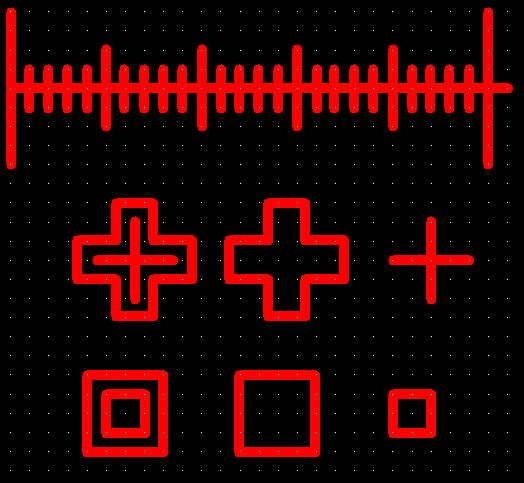
\includegraphics[scale=0.25]{mask-art.png}
\end{center}
\caption{Mask art used in tests. All lines are 1 $\lambda$ wide.}
\label{mask-art}
\end{figure}

\subsection{Experiment 1 - Photo Tube}

\begin{figure}[h]
\begin{center}
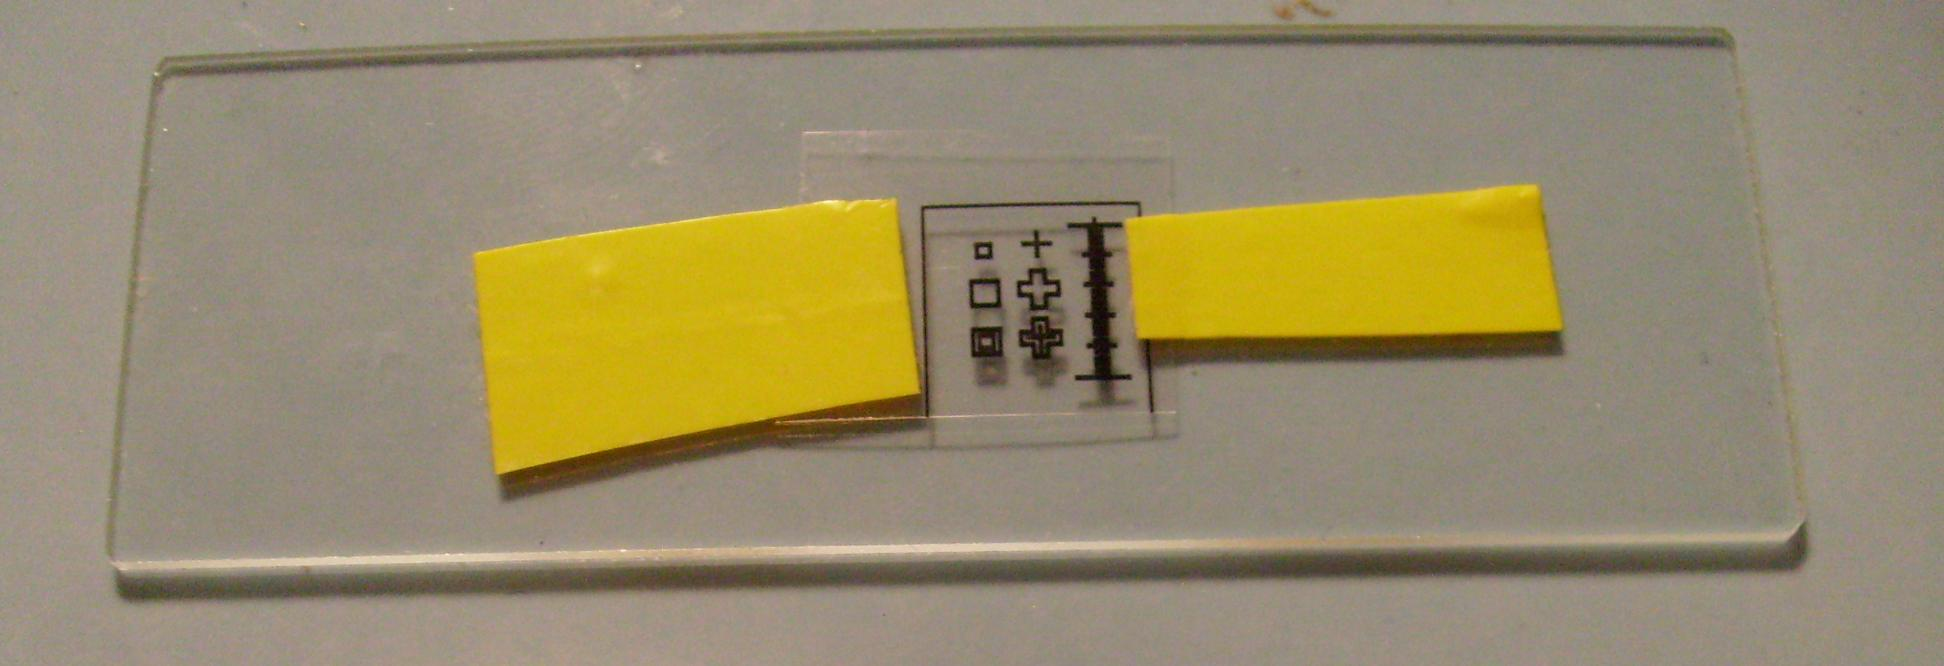
\includegraphics[scale=0.1]{mask-art-2.jpg}
\end{center}
\caption{Mask art printed at $\lambda = 150 \mu m$ and mounted on microscope slide. Note blurring of adjacent lines.}
\label{mask-art-2}
\end{figure}

\begin{figure}[h]
\begin{center}
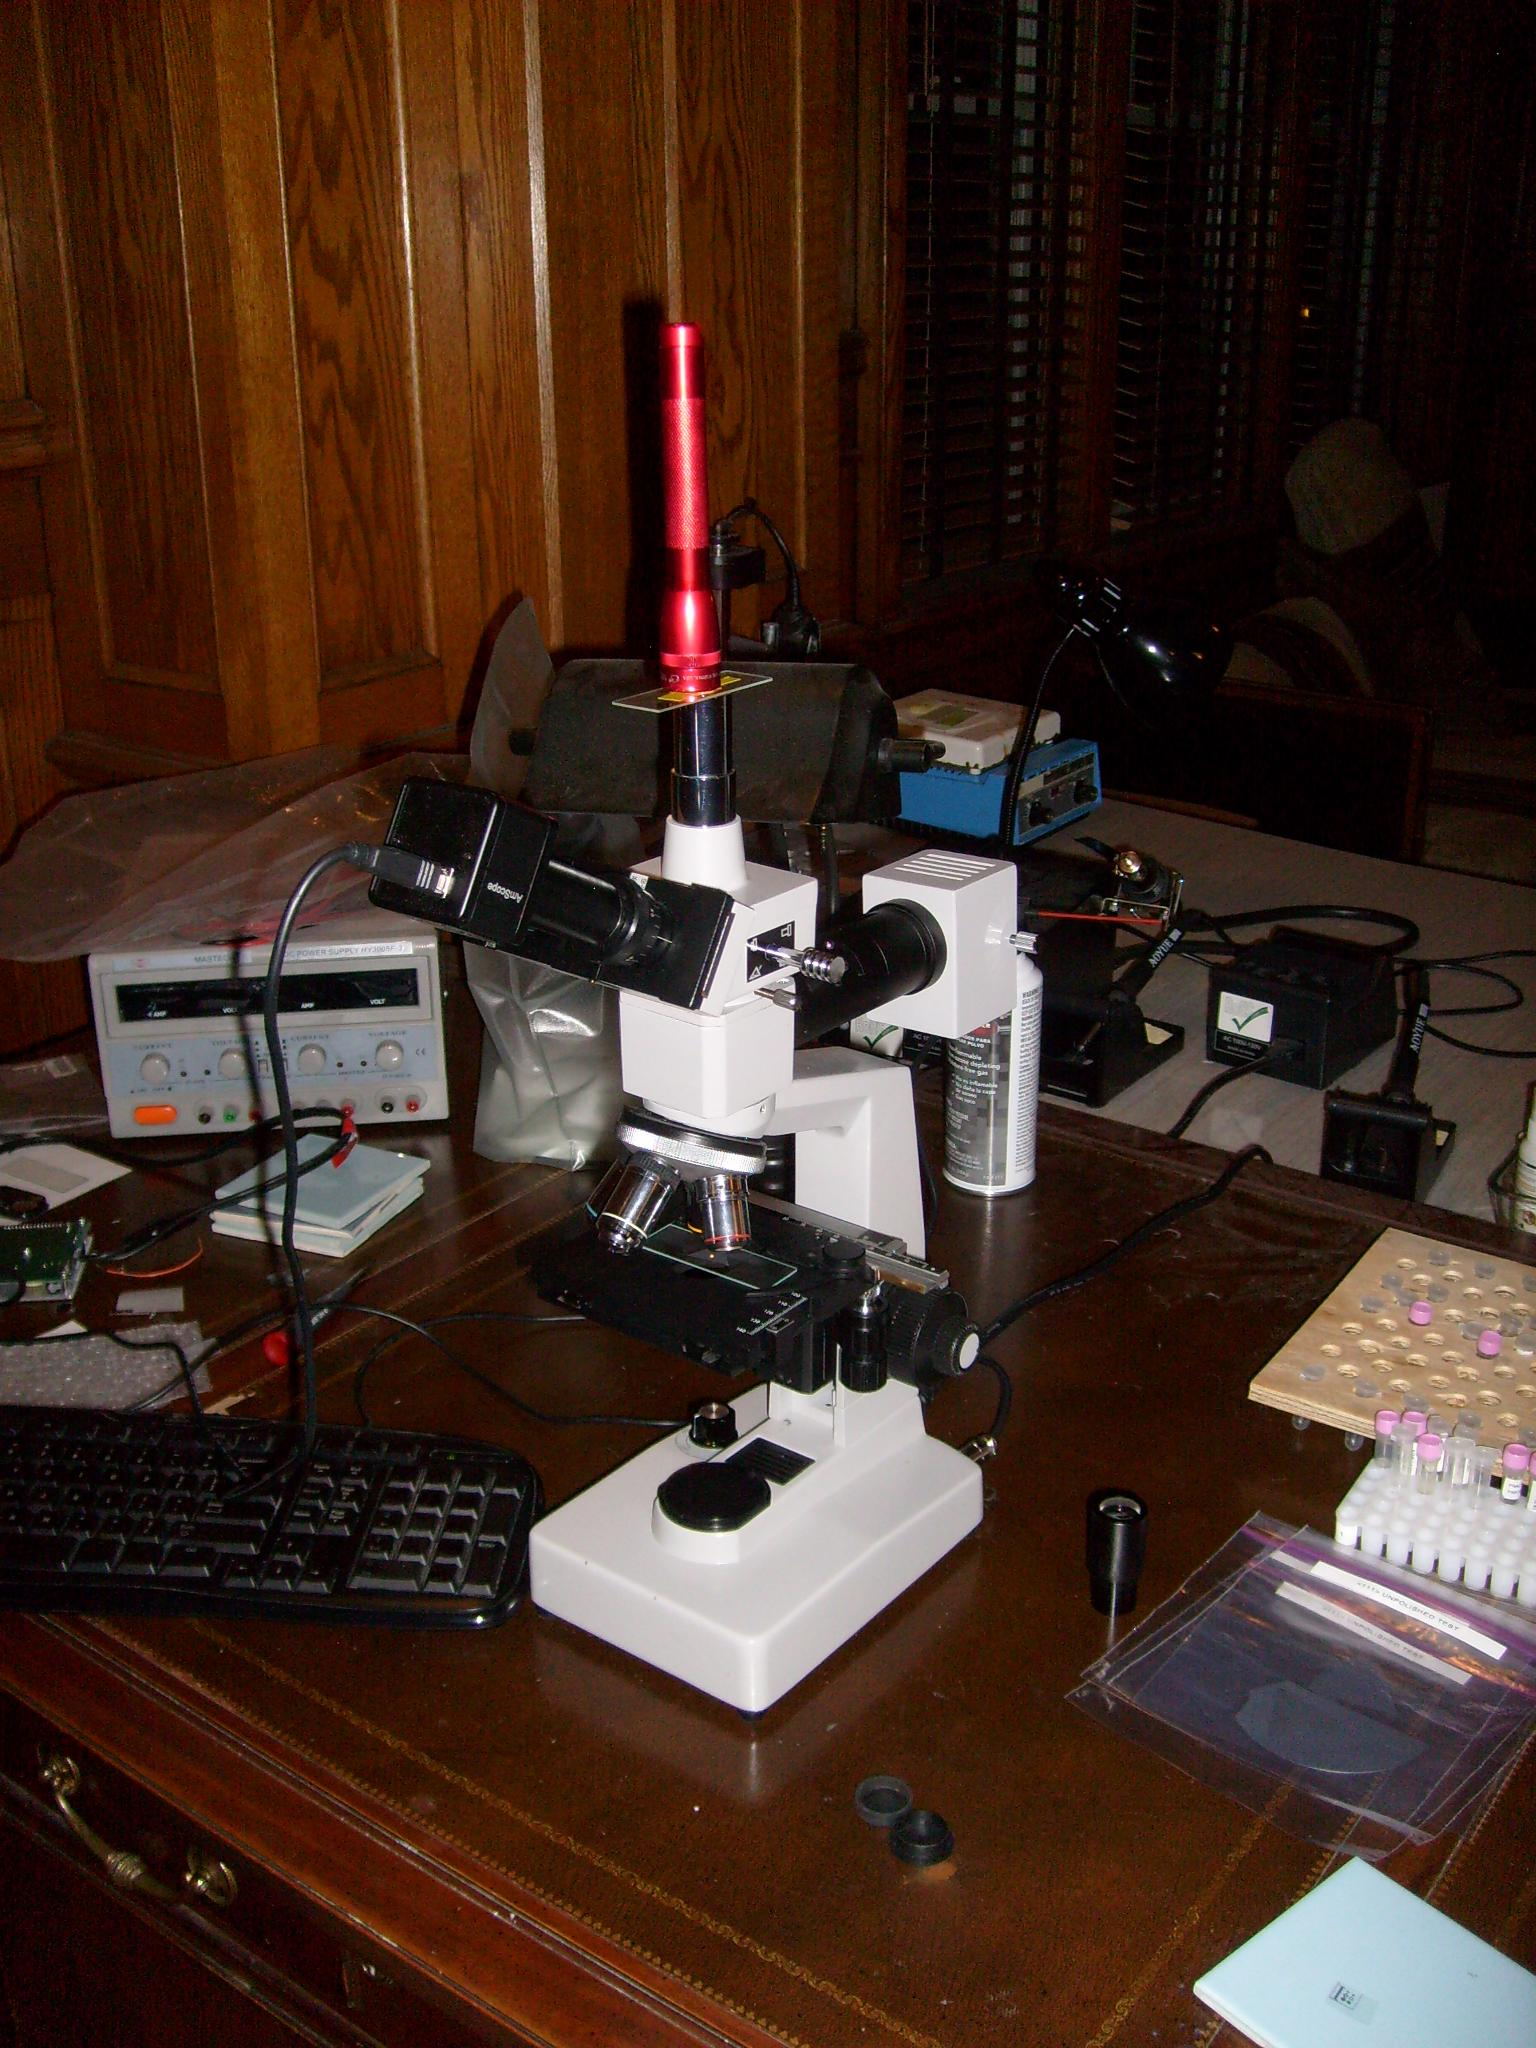
\includegraphics[scale=0.1]{first-test.jpg}
\end{center}
\caption{Initial experimental setup.}
\label{first-test}
\end{figure}


\begin{figure}[h]
\begin{center}
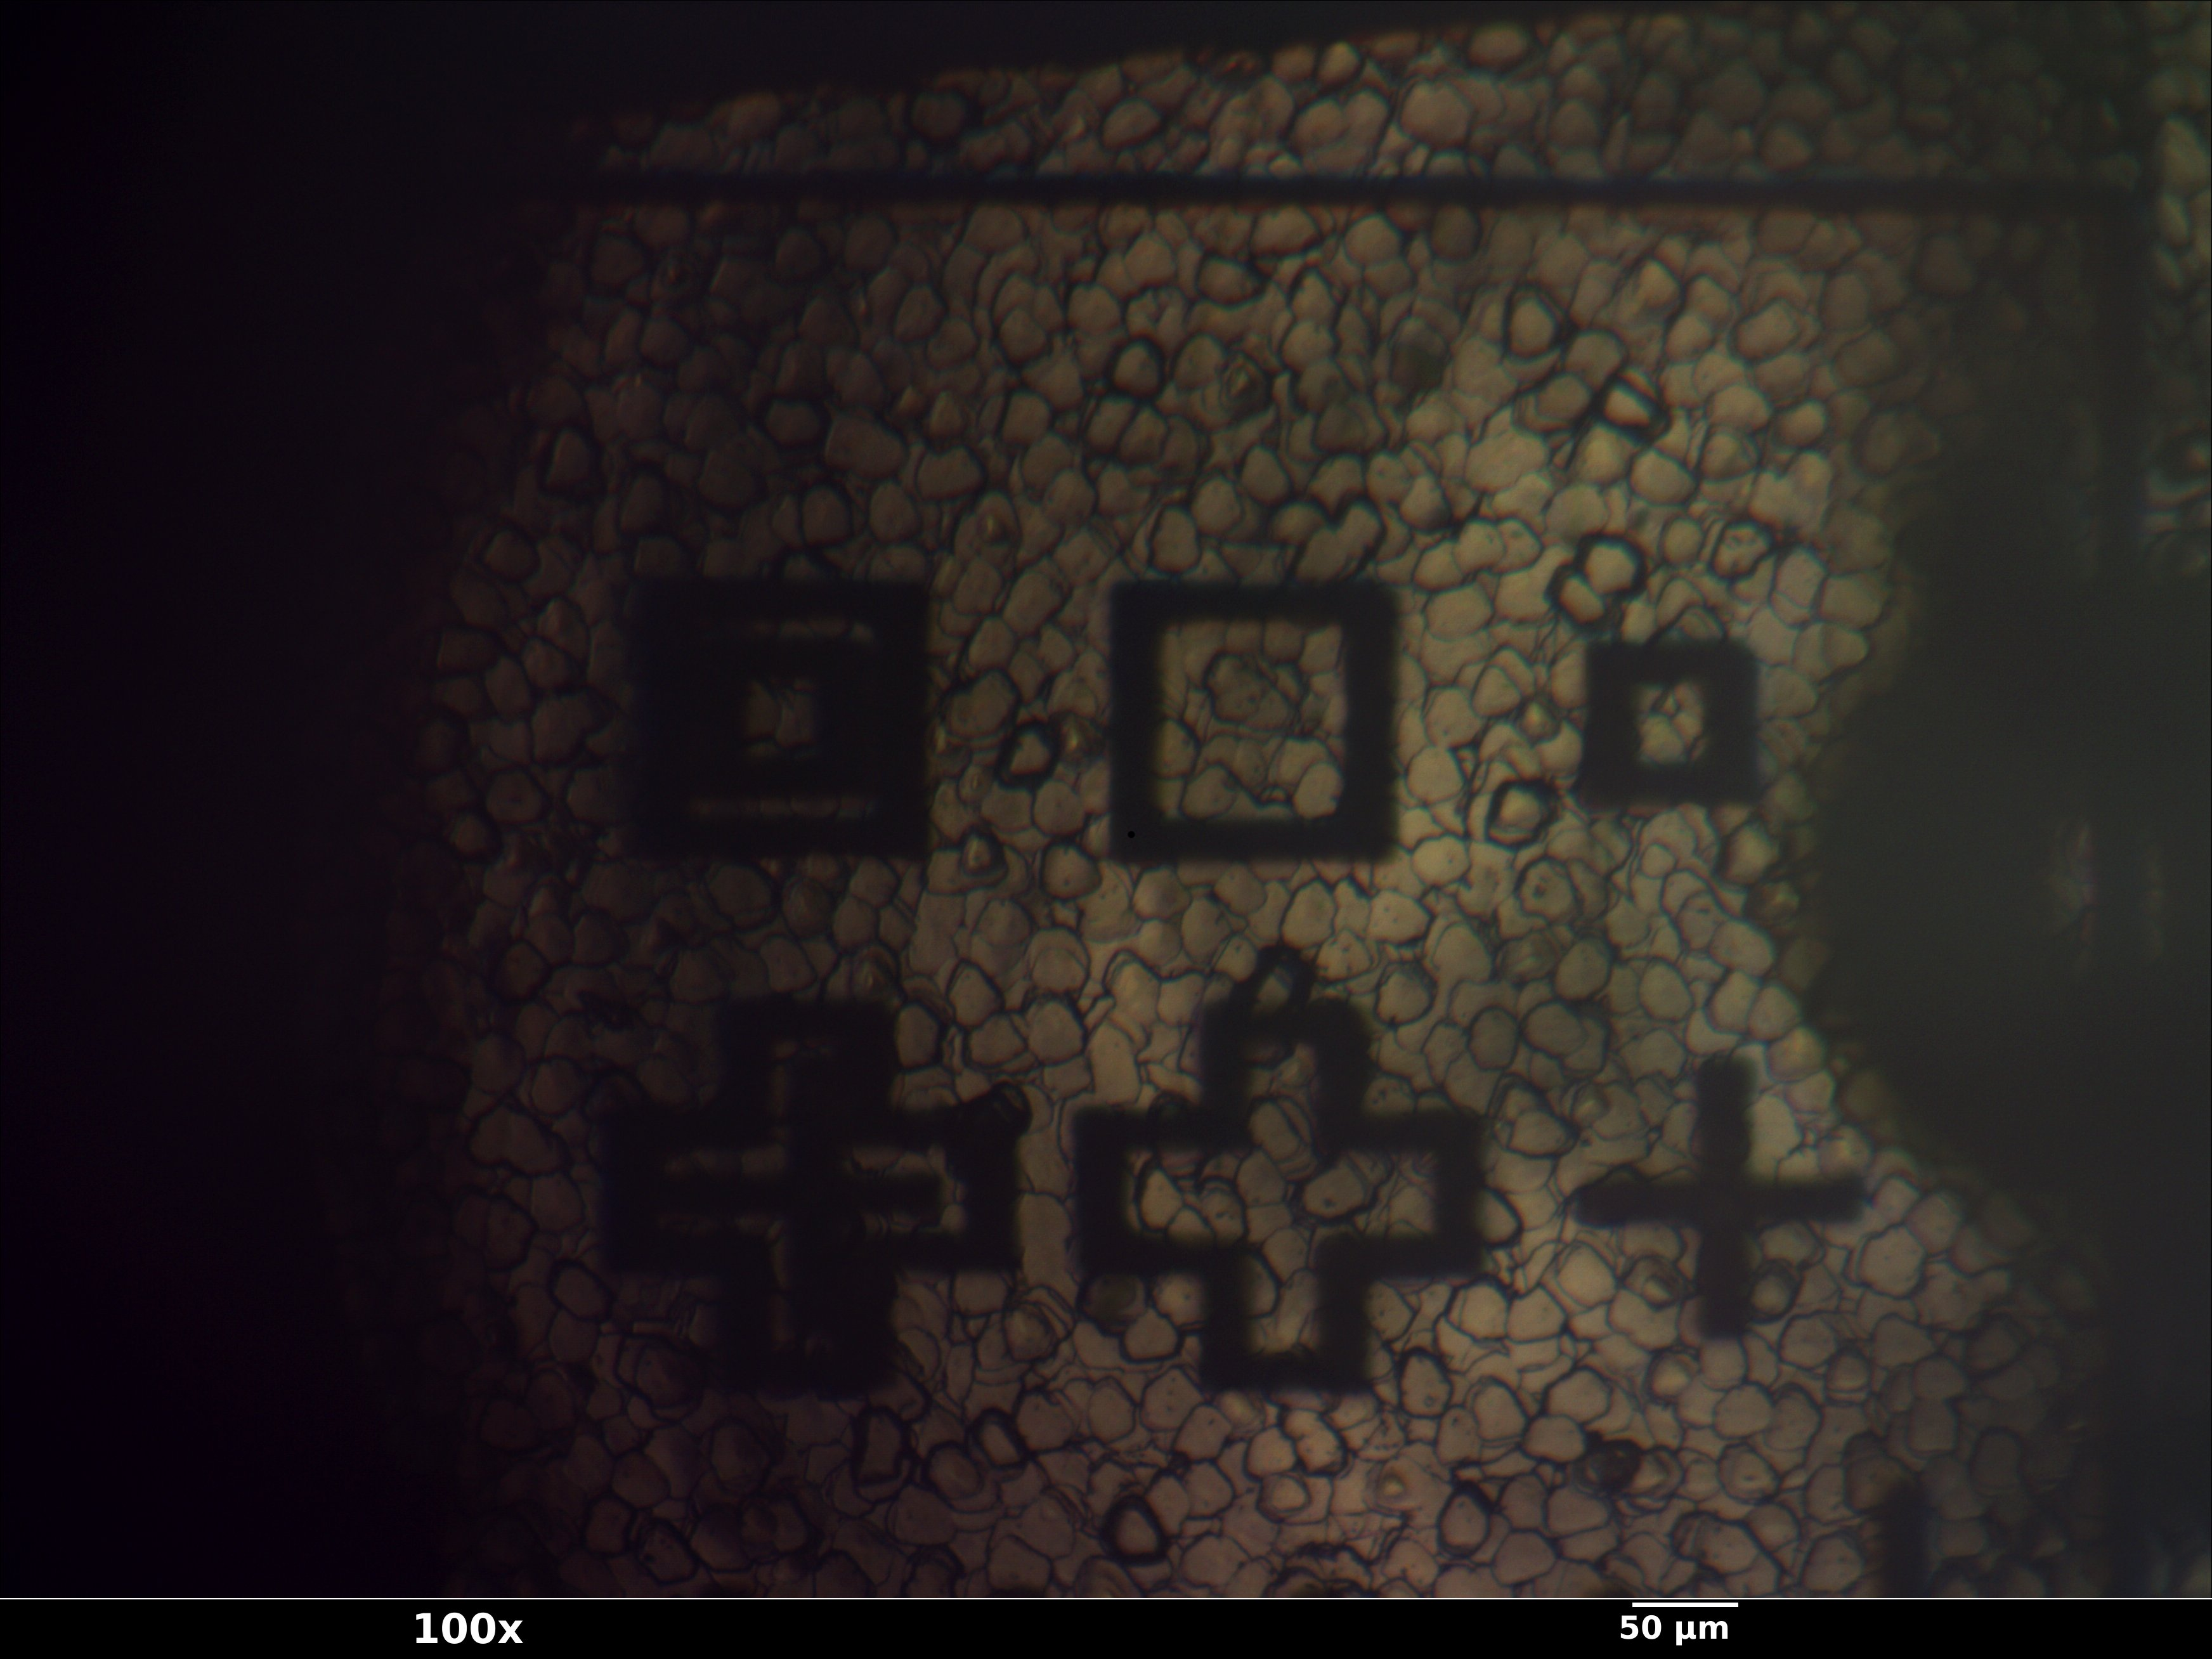
\includegraphics[scale=0.06]{mask001_annotated.jpg}
\end{center}
\caption{The first test, using 10x objective. Substrate is unpolished $<111>$ Si wafer. Note extremely poor
illumination.}
\label{first-test-close}
\end{figure}

\paragraph*{}
The first test used the mask art shown in Fig. ~\ref{mask-art} printed at $\lambda = 150 \mu m$ (Fig.
~\ref{mask-art-2}). The mask art was placed on top of the photo tube of the microscope and illuminated with an AA
Mag-Lite (Fig. ~\ref{first-test}).

\paragraph*{}
Reduction by the objective's magnification was observed with 4x/10x/40x objectives. (The microscope was also equipped
with a 100x oil immersion objective which was not tested). Illumination was extremely uneven and dim, and not suitable
for lithographic purposes.

\paragraph*{}
The most obvious problem with this setup is the poor illumination. (The fact that a pocket flashlight was being used
instead of a proper collimated light source is certainly responsible in part!) The resulting stack is also difficult
to keep stable and will require some sort of bracket. Due to these difficulties the author abandoned this method
and went on to another design. He intends to return and explore this method in more detail in a future paper.

\paragraph*{}
Another issue noted was the blurring of adjacent lines on the actual mask art printout. It was determined that $150
\mu m$ was too small for the printer used to resolved reliably.

\subsection{Experiment 2 - Epi-Illuminator}
\paragraph*{}
The next experiment was intended to correct the illumination problems exhibited by the first method. The illuminator 
tube was disassembled and the diaphragm assembly removed. Mask art was inserted through a slit in the tube and placed
at the focal point of the illuminator (Fig. ~\ref{second-test}). This mask was printed at $\lambda = 200 \mu m$ to avoid
the printer-resolution issues observed in the first test.

\begin{figure}[h]
\begin{center}
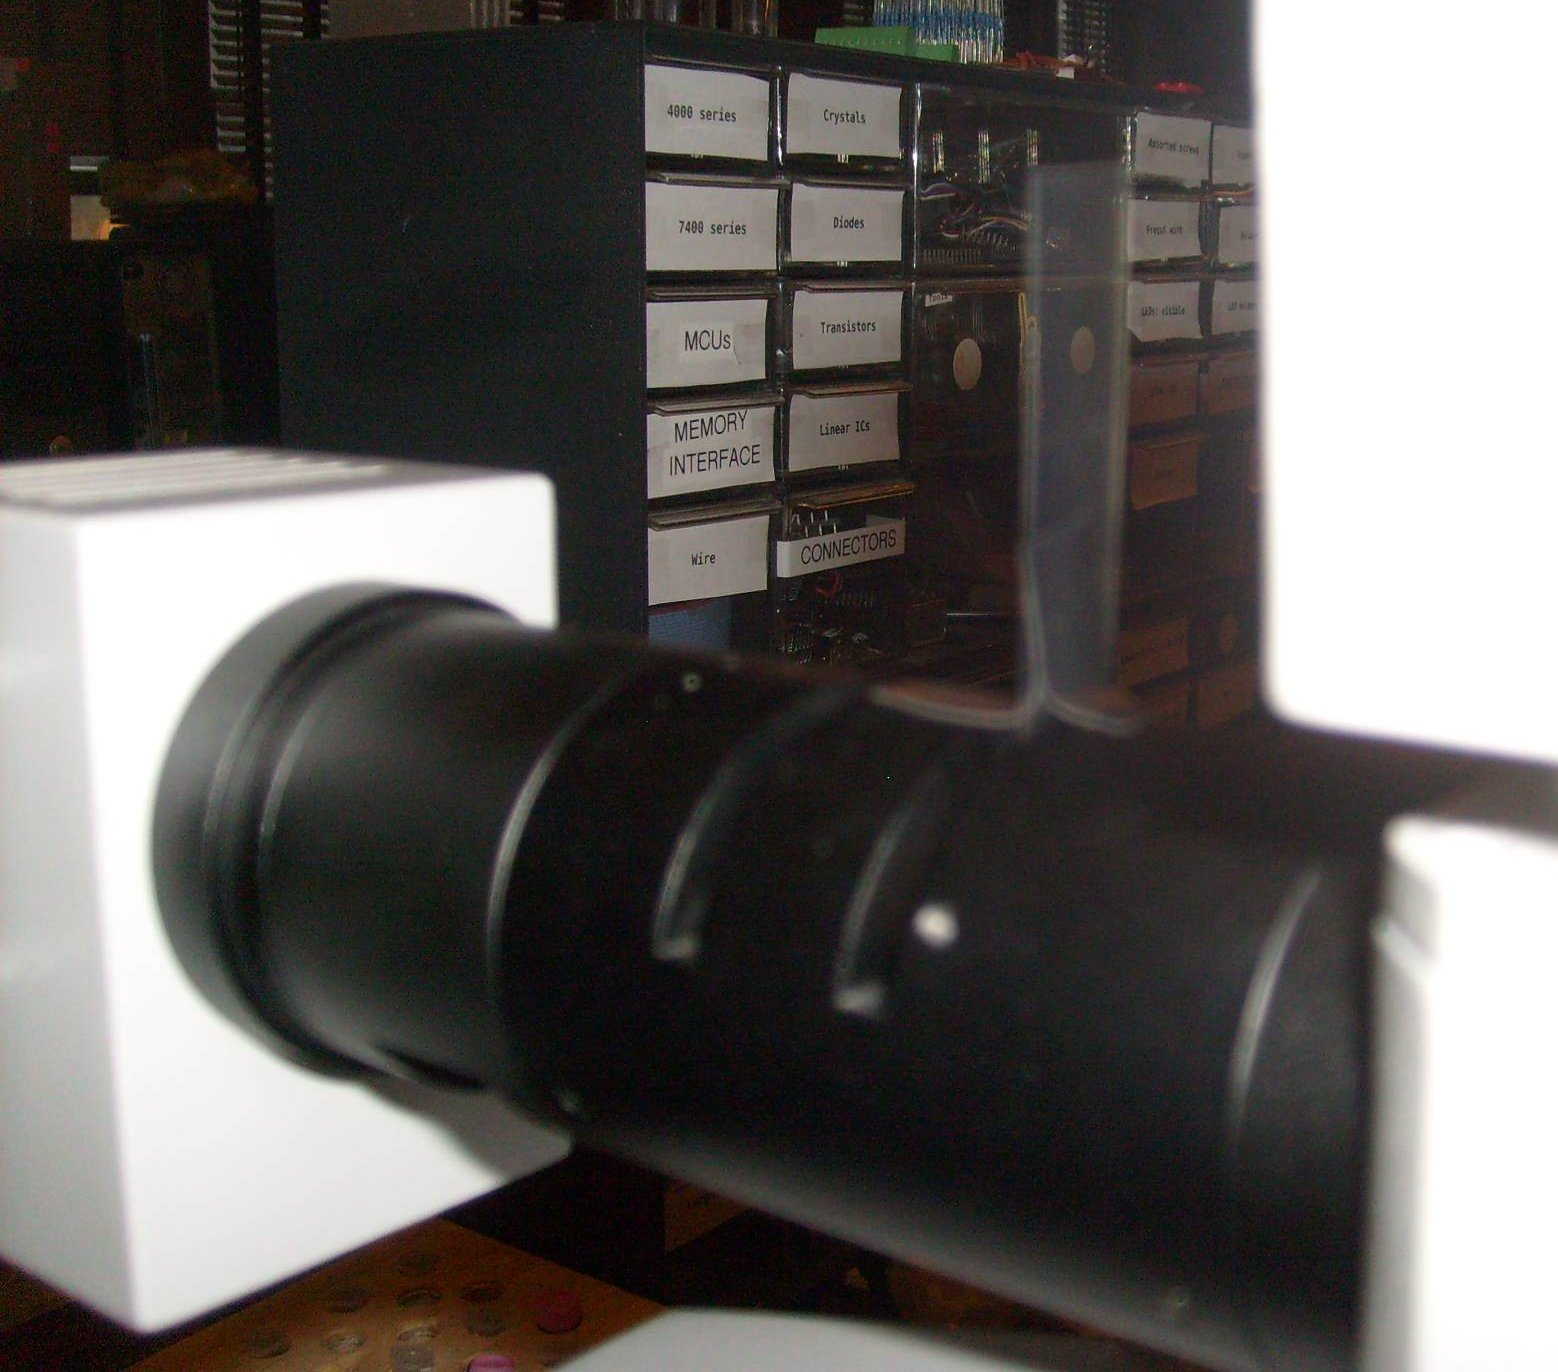
\includegraphics[scale=0.1]{second-test.jpg}
\end{center}
\caption{Mask art mounted inside epi-illuminator for second test}
\label{second-test}
\end{figure}

\begin{figure}[h]
\begin{center}
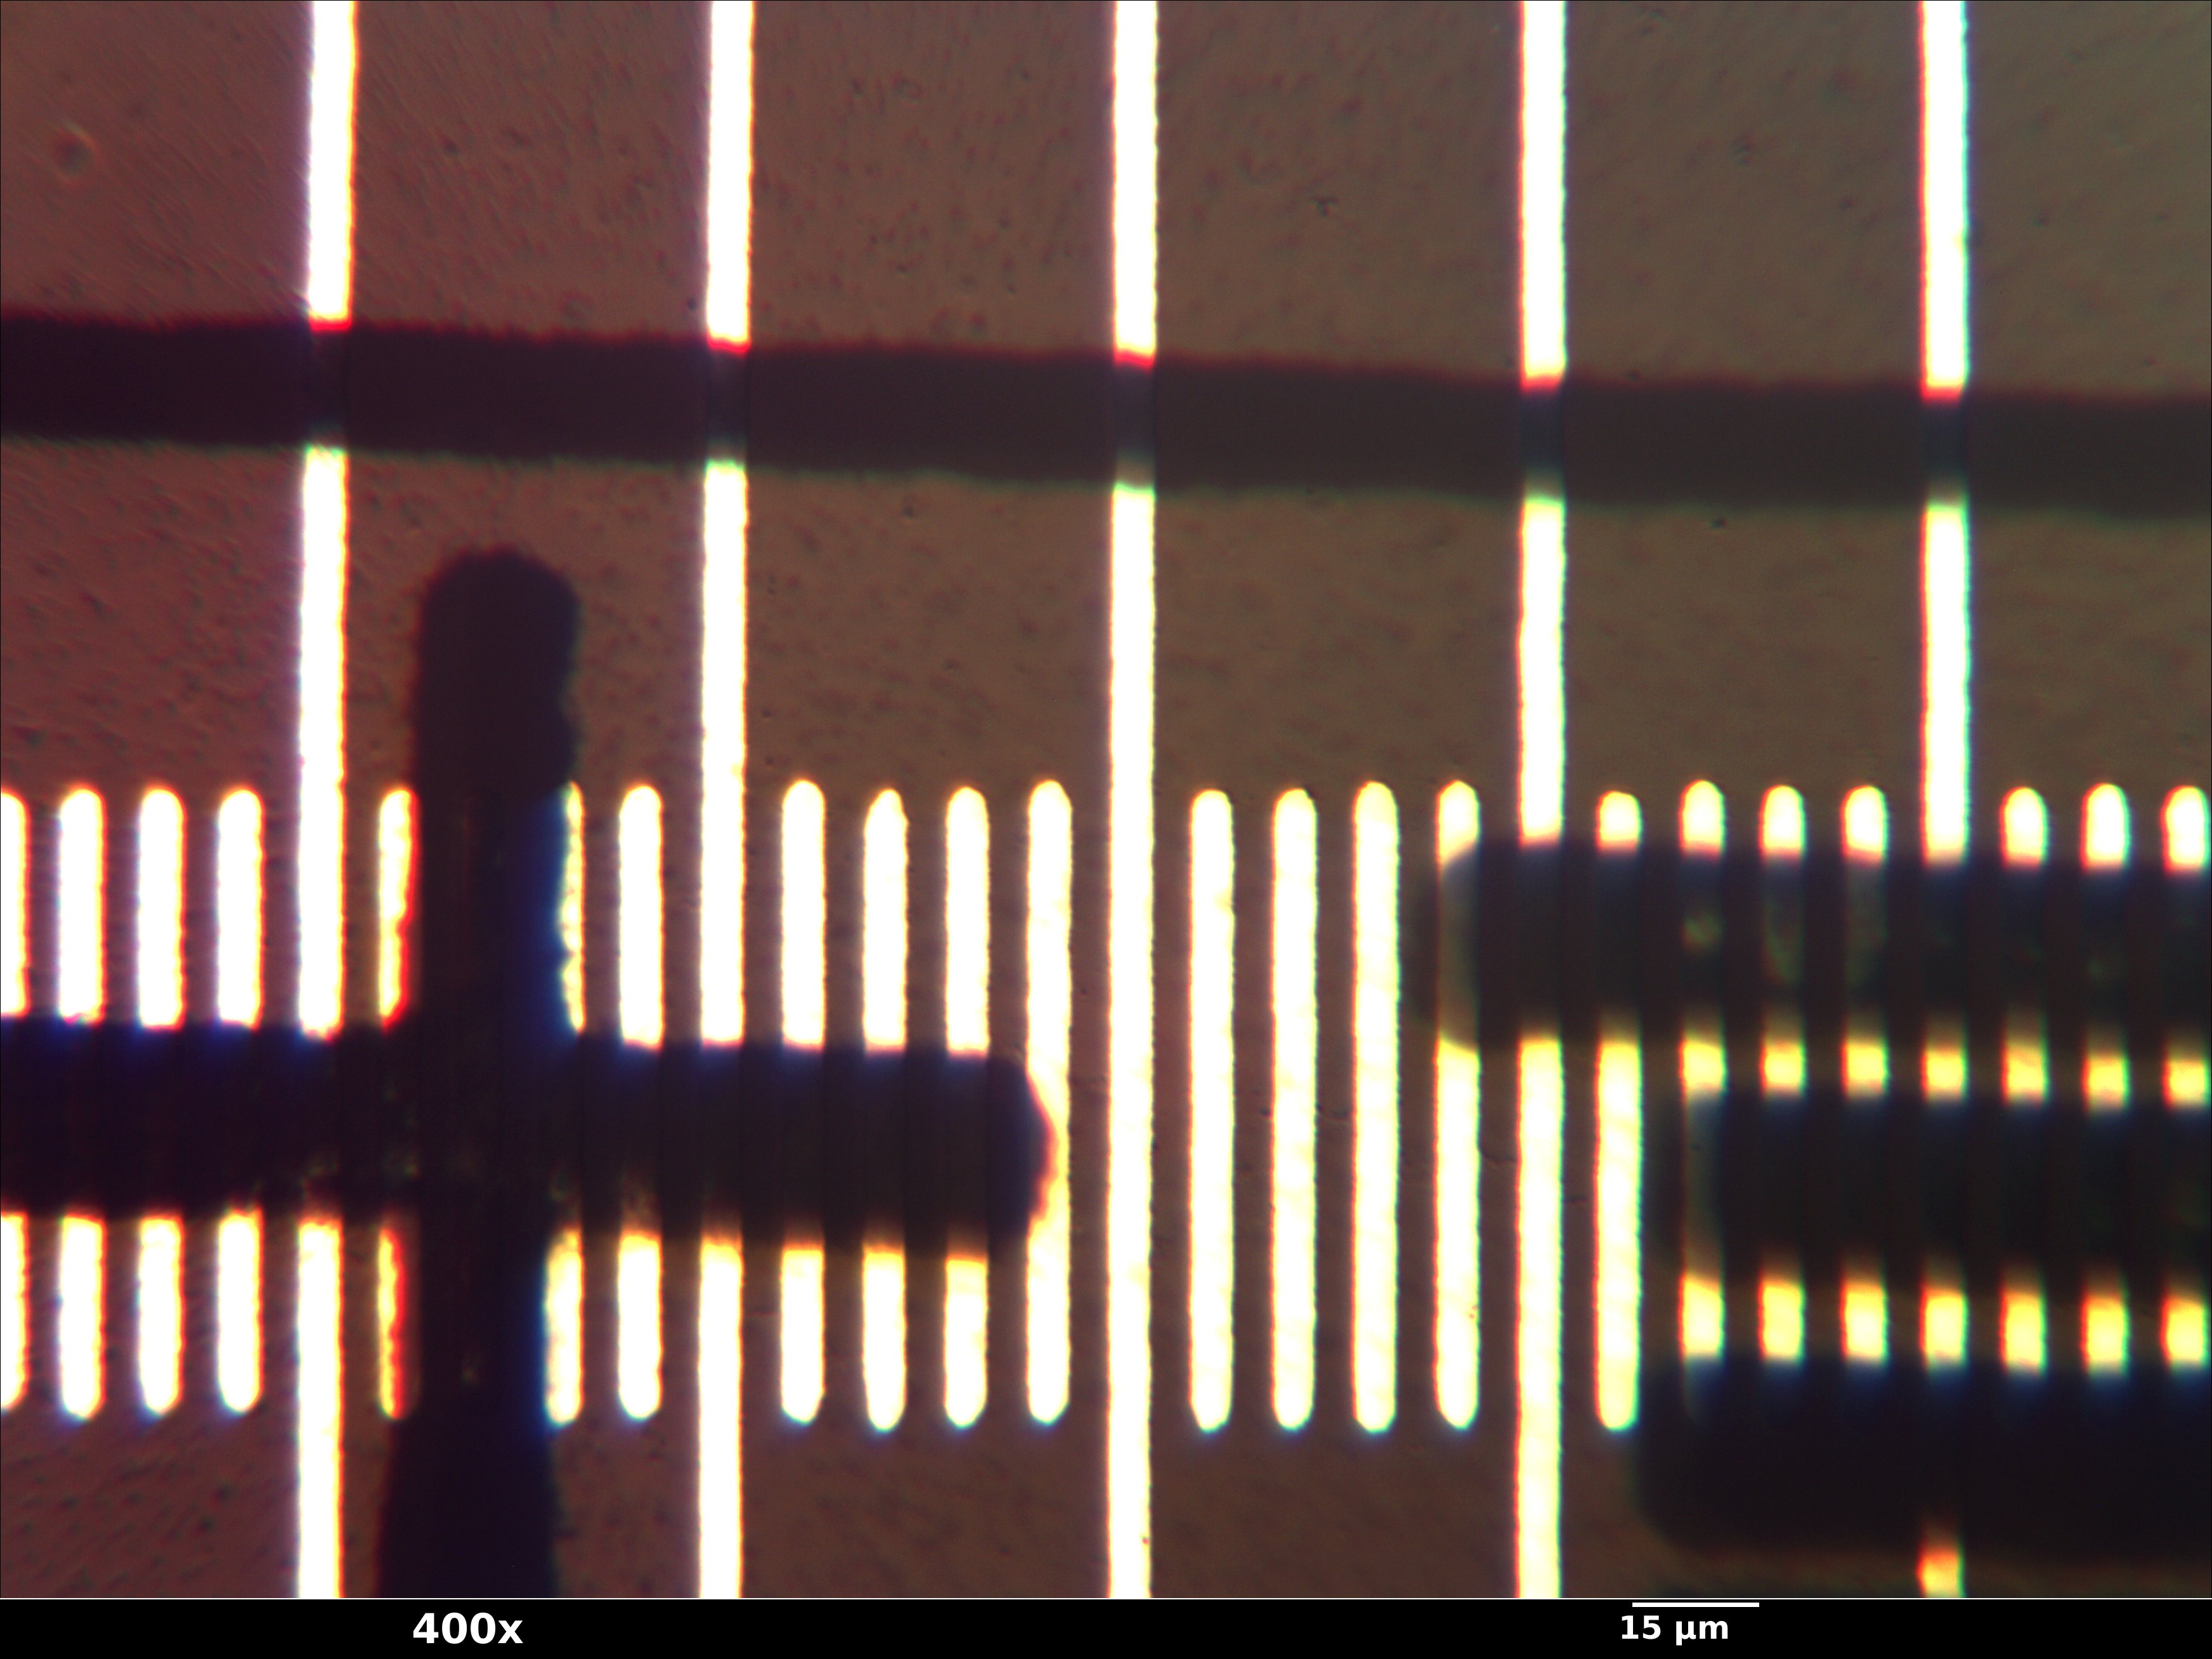
\includegraphics[scale=0.06]{mask004_annotated.jpg}
\end{center}
\caption{View of improved illumination on test pattern, projected onto stage micrometer with 40x objective. Note 3x
less reduction compared to first experiment. Minor scale divisions are $10 \mu m$.}
\label{second-test-close}
\end{figure}

\paragraph*{}
Illumination was much improved compared to the first test (Fig. ~\ref{second-test-close}), however since the pattern was
inserted lower in the optical path the reduction factor was less than that of the first method (approximately objective
magnification/3).

\paragraph*{}
At this point it was decided the technique was sufficiently mature to warrant actual lithography tests. The mask was 
projected with the 40x objective onto a piece of Datak printed circuit board pre-coated with dry-film photoresist and
focused under subdued light. The illuminator was then turned up to full scale and the sample exposed for 15 minutes.
After exposure was completed the sample was developed in a 100:1 weight solution of NaOH crystals in distilled water,
followed by a distilled water rinse.

\begin{figure}[h]
\begin{center}
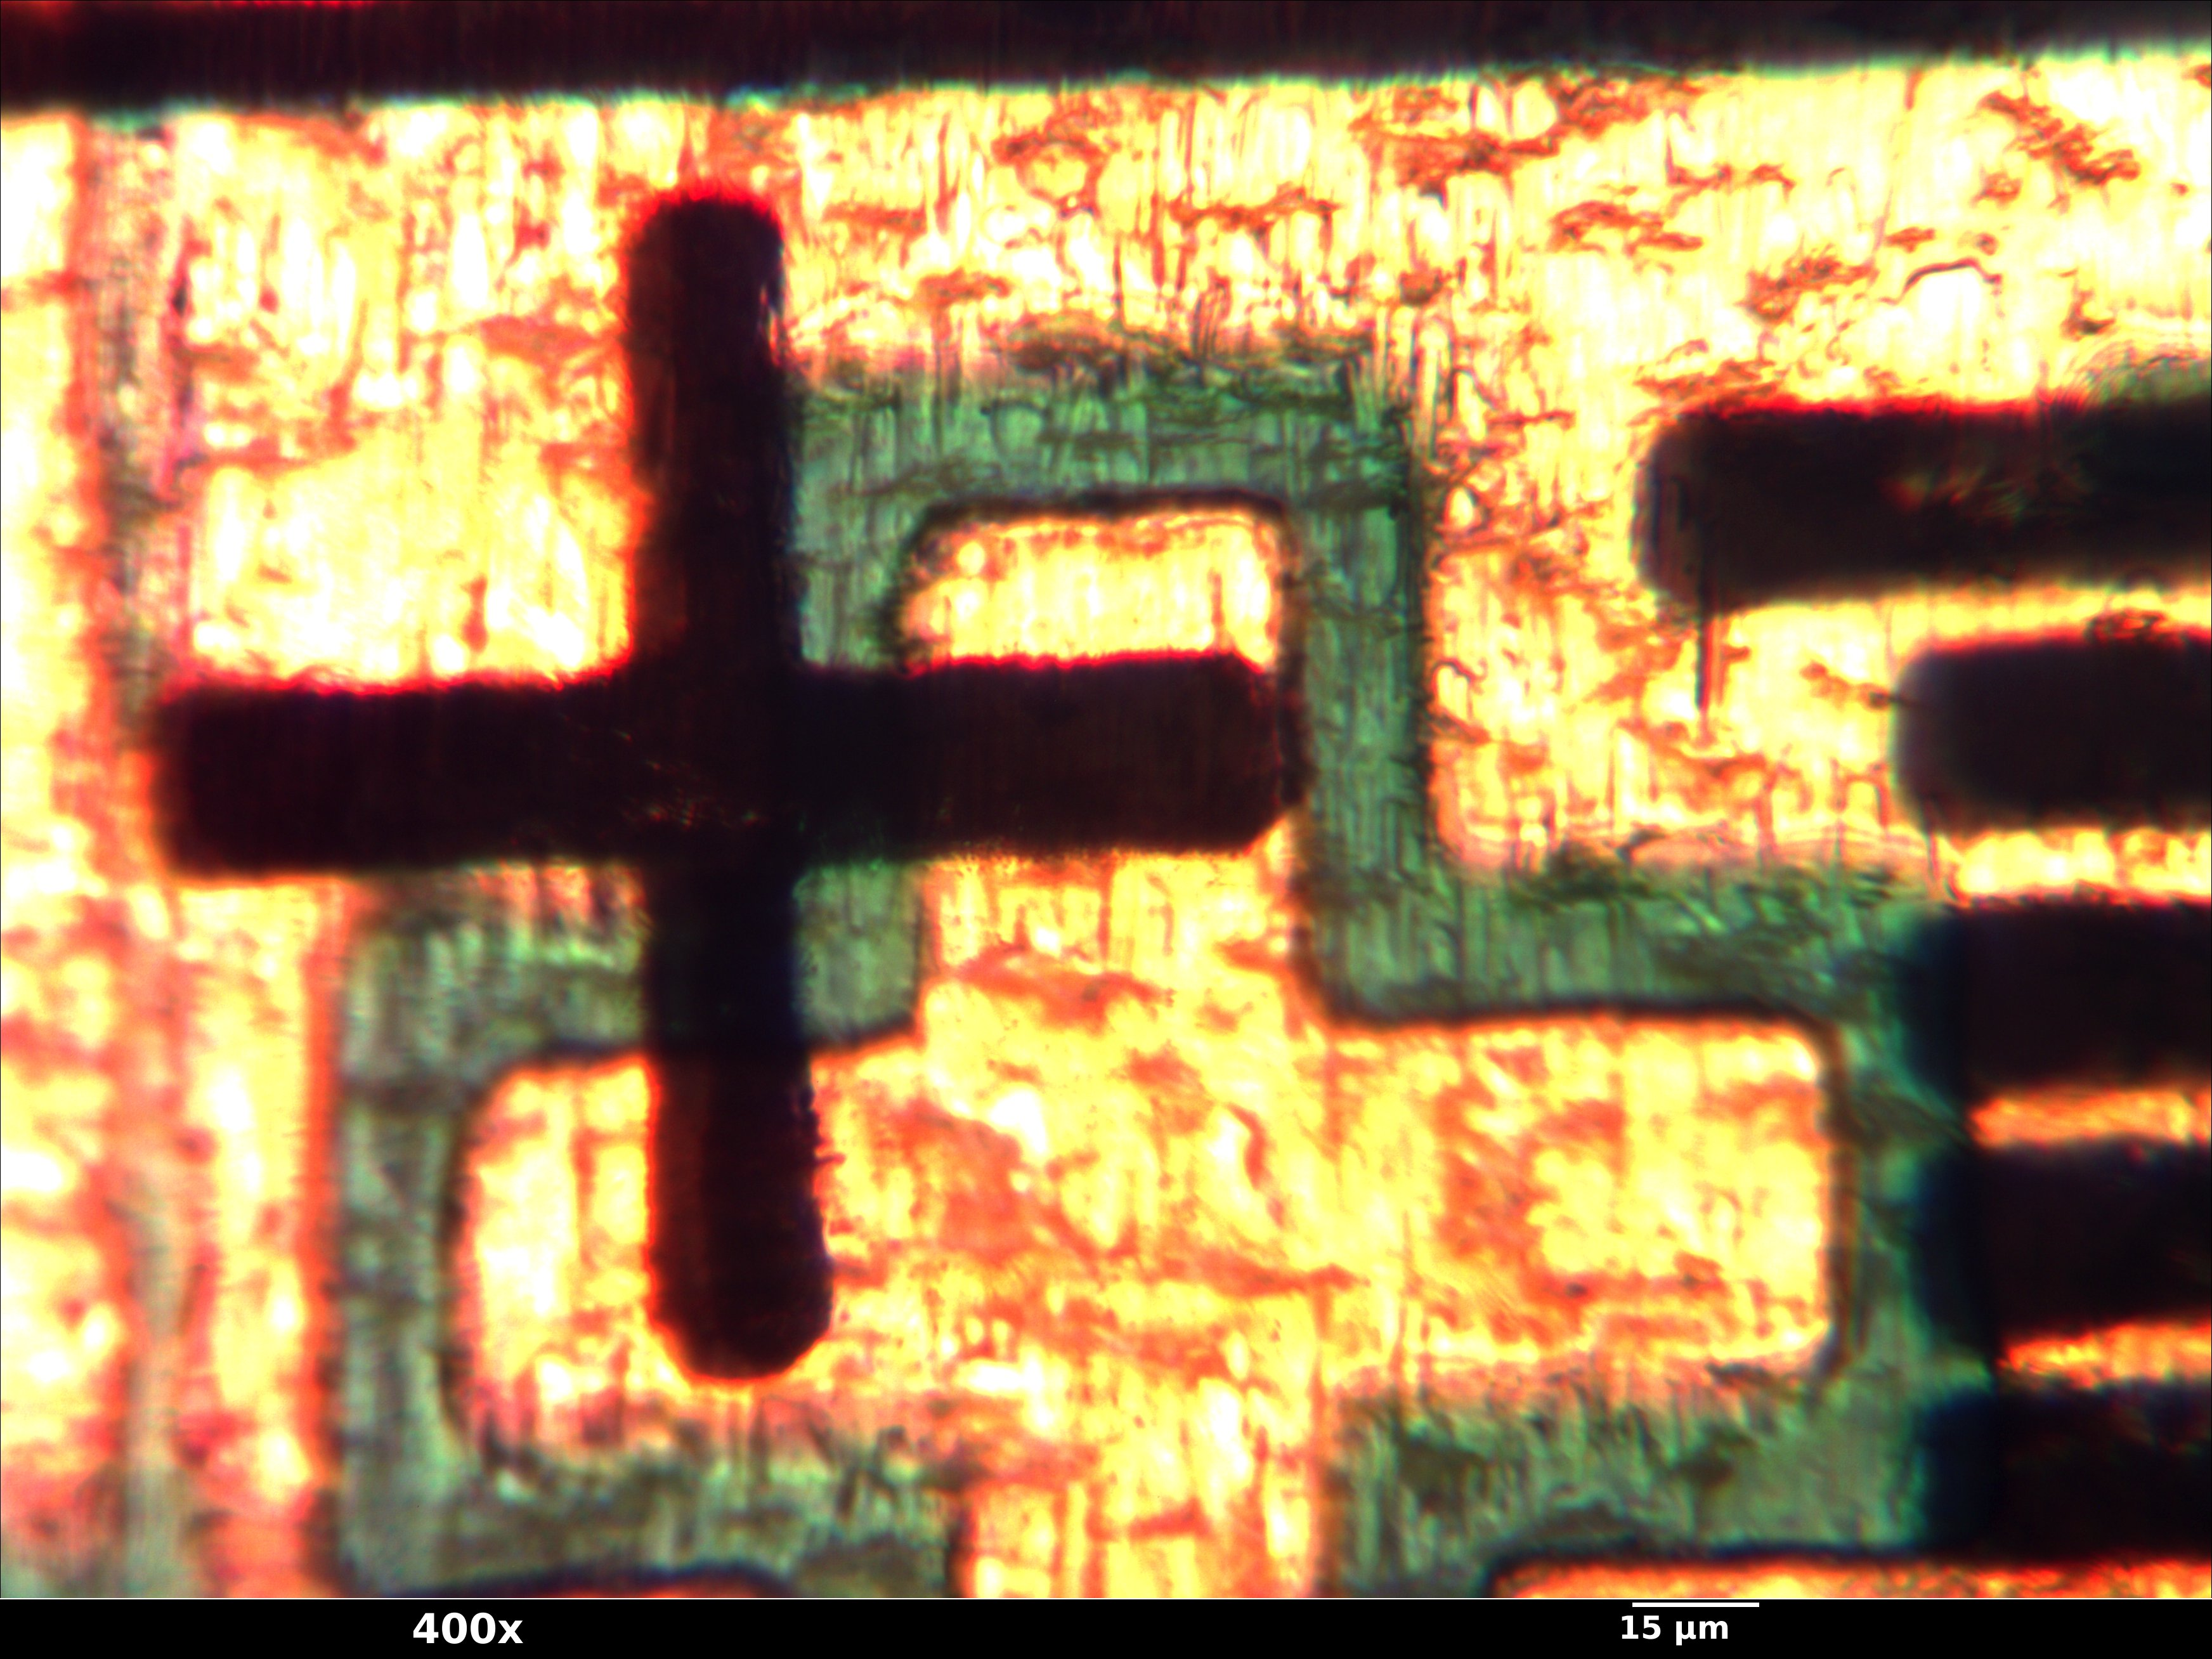
\includegraphics[scale=0.06]{mask010_annotated.jpg}
\end{center}
\caption{Developed pattern (positive photoresist on copper) before alignment to second-level mask art.}
\label{alignment-1}
\end{figure}

\begin{figure}[h!]
\begin{center}
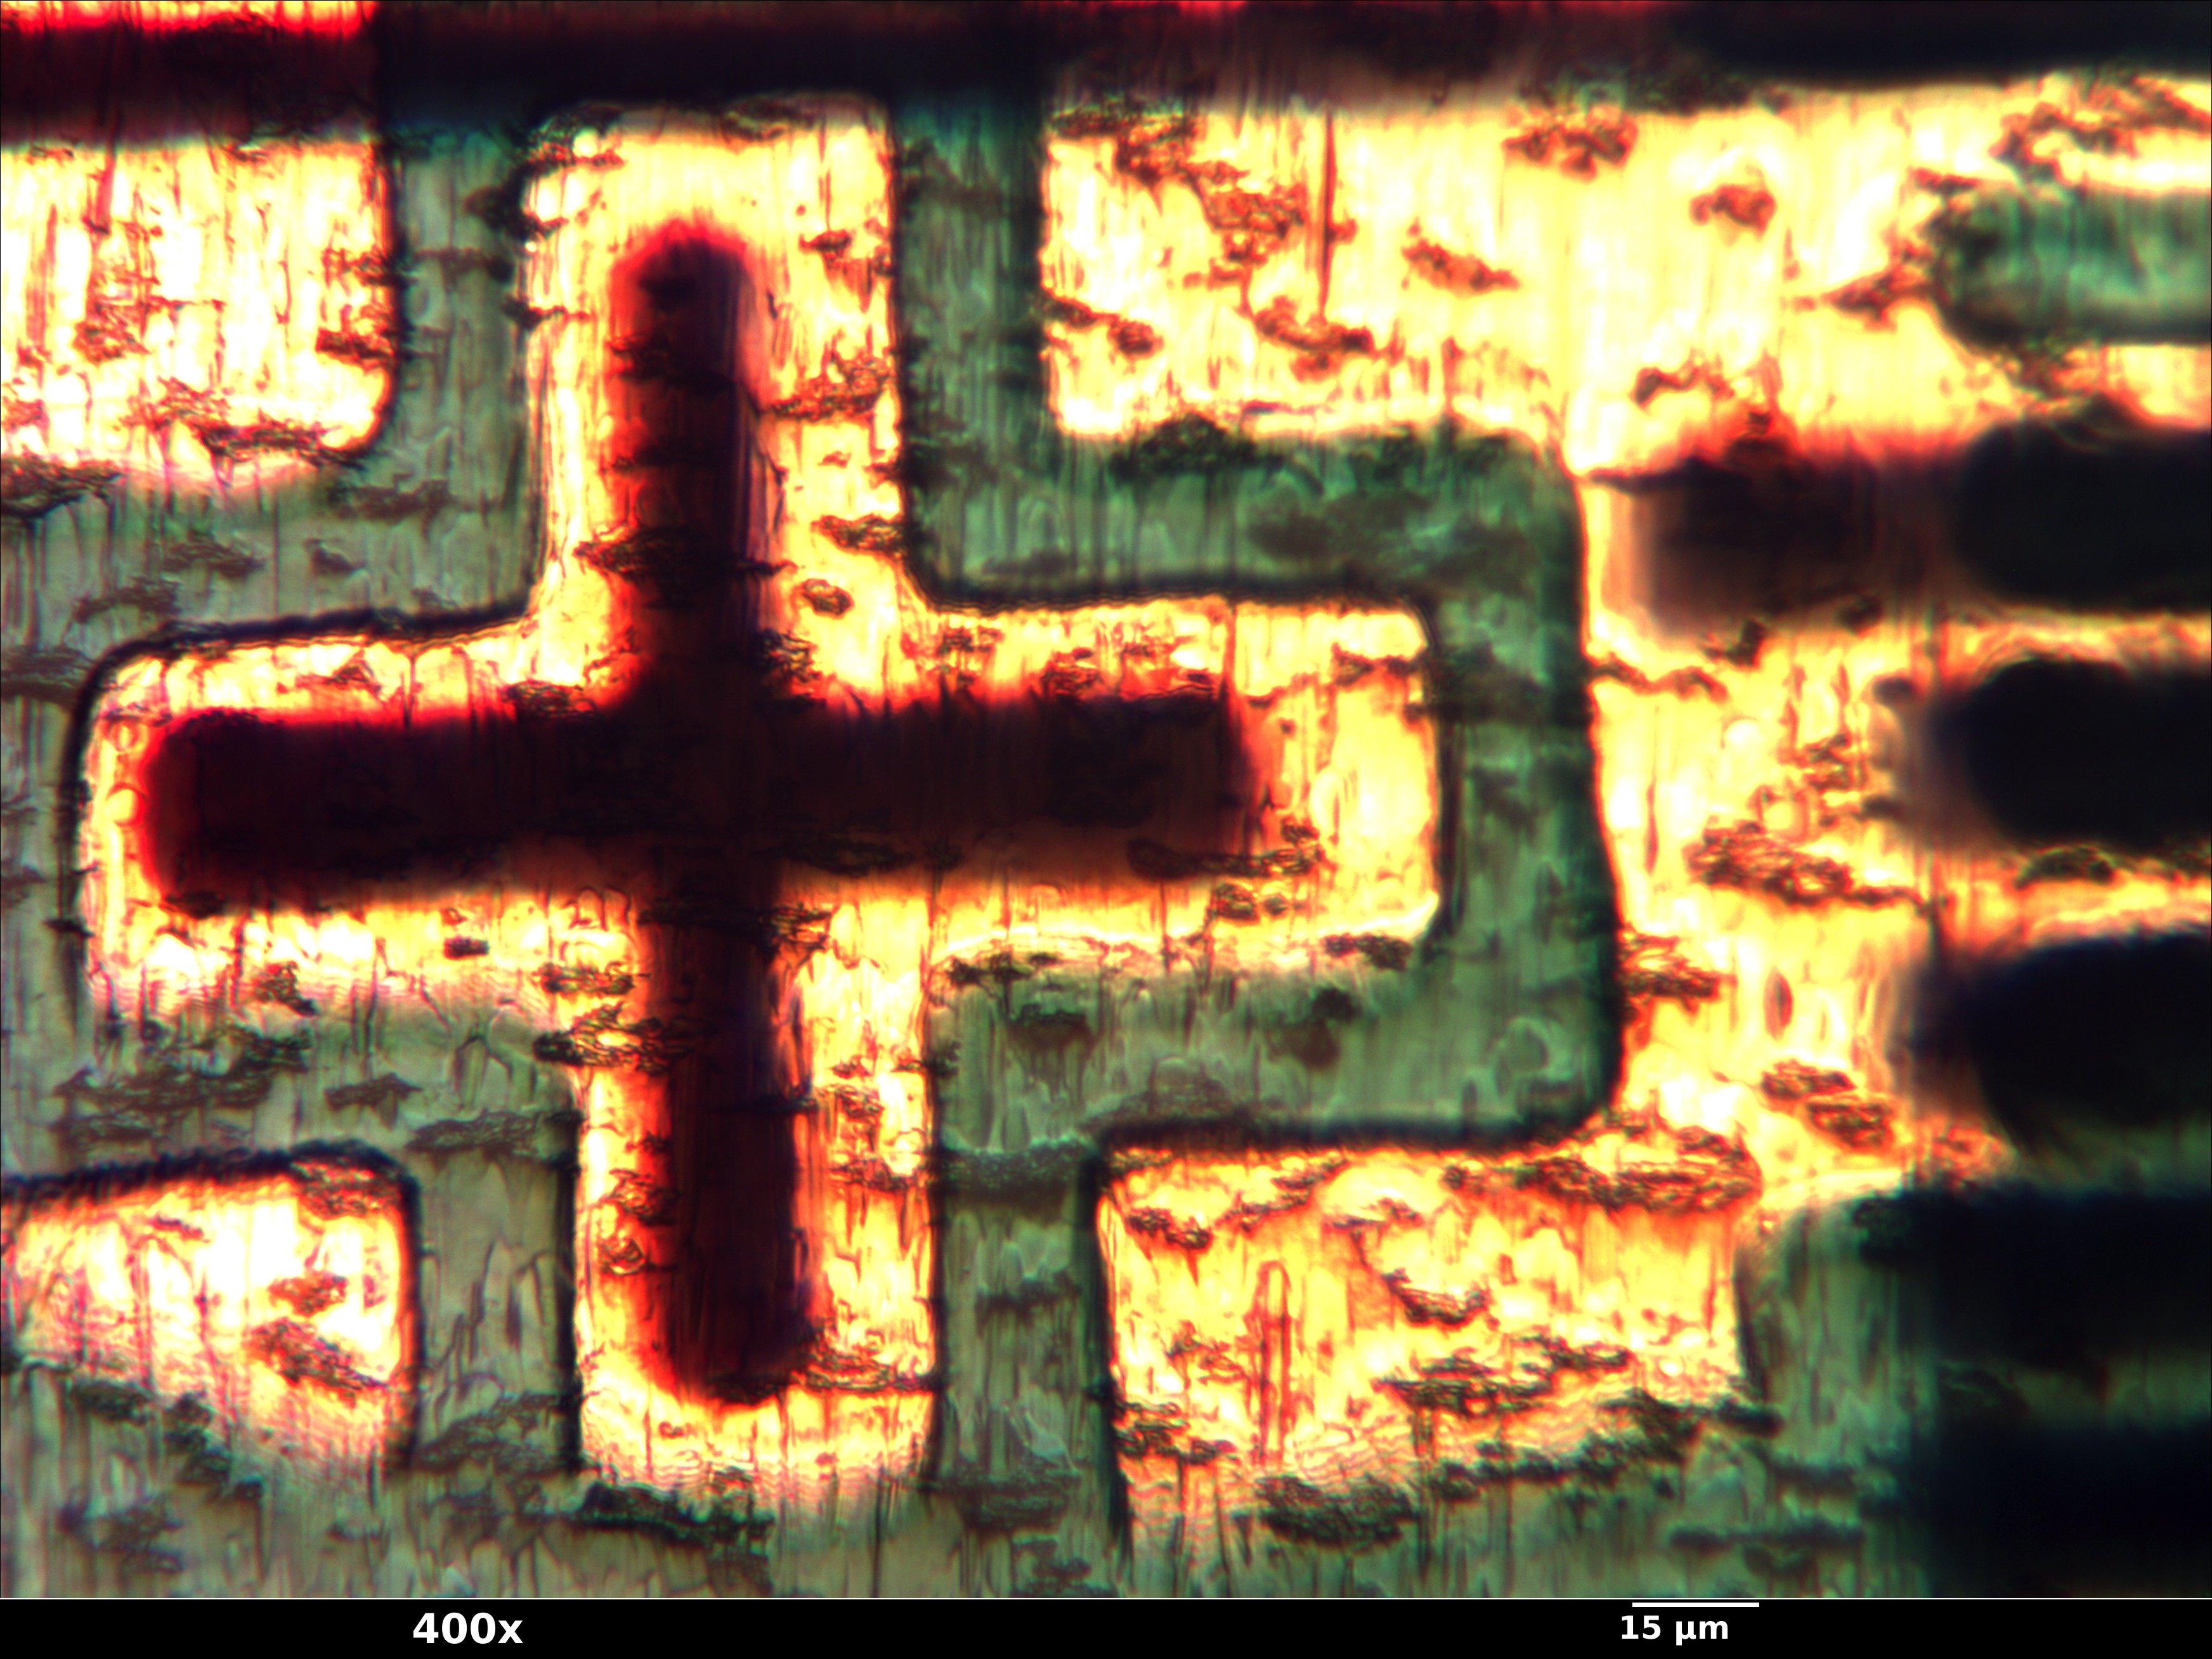
\includegraphics[scale=0.06]{mask009_annotated.jpg}
\end{center}
\caption{Developed pattern after alignment to second-level mask art.}
\label{alignment-2}
\end{figure}

\begin{figure}[h!]
\begin{center}
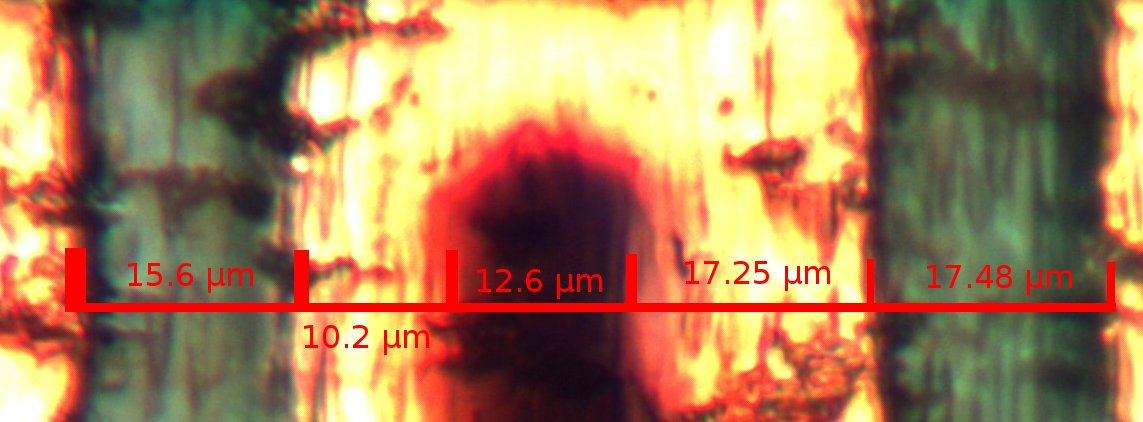
\includegraphics[scale=0.15]{mask009_annotated2.jpg}
\end{center}
\caption{Pitch measurements on the sample.}
\label{pitch}
\end{figure}

\begin{figure}[h!]
\begin{center}
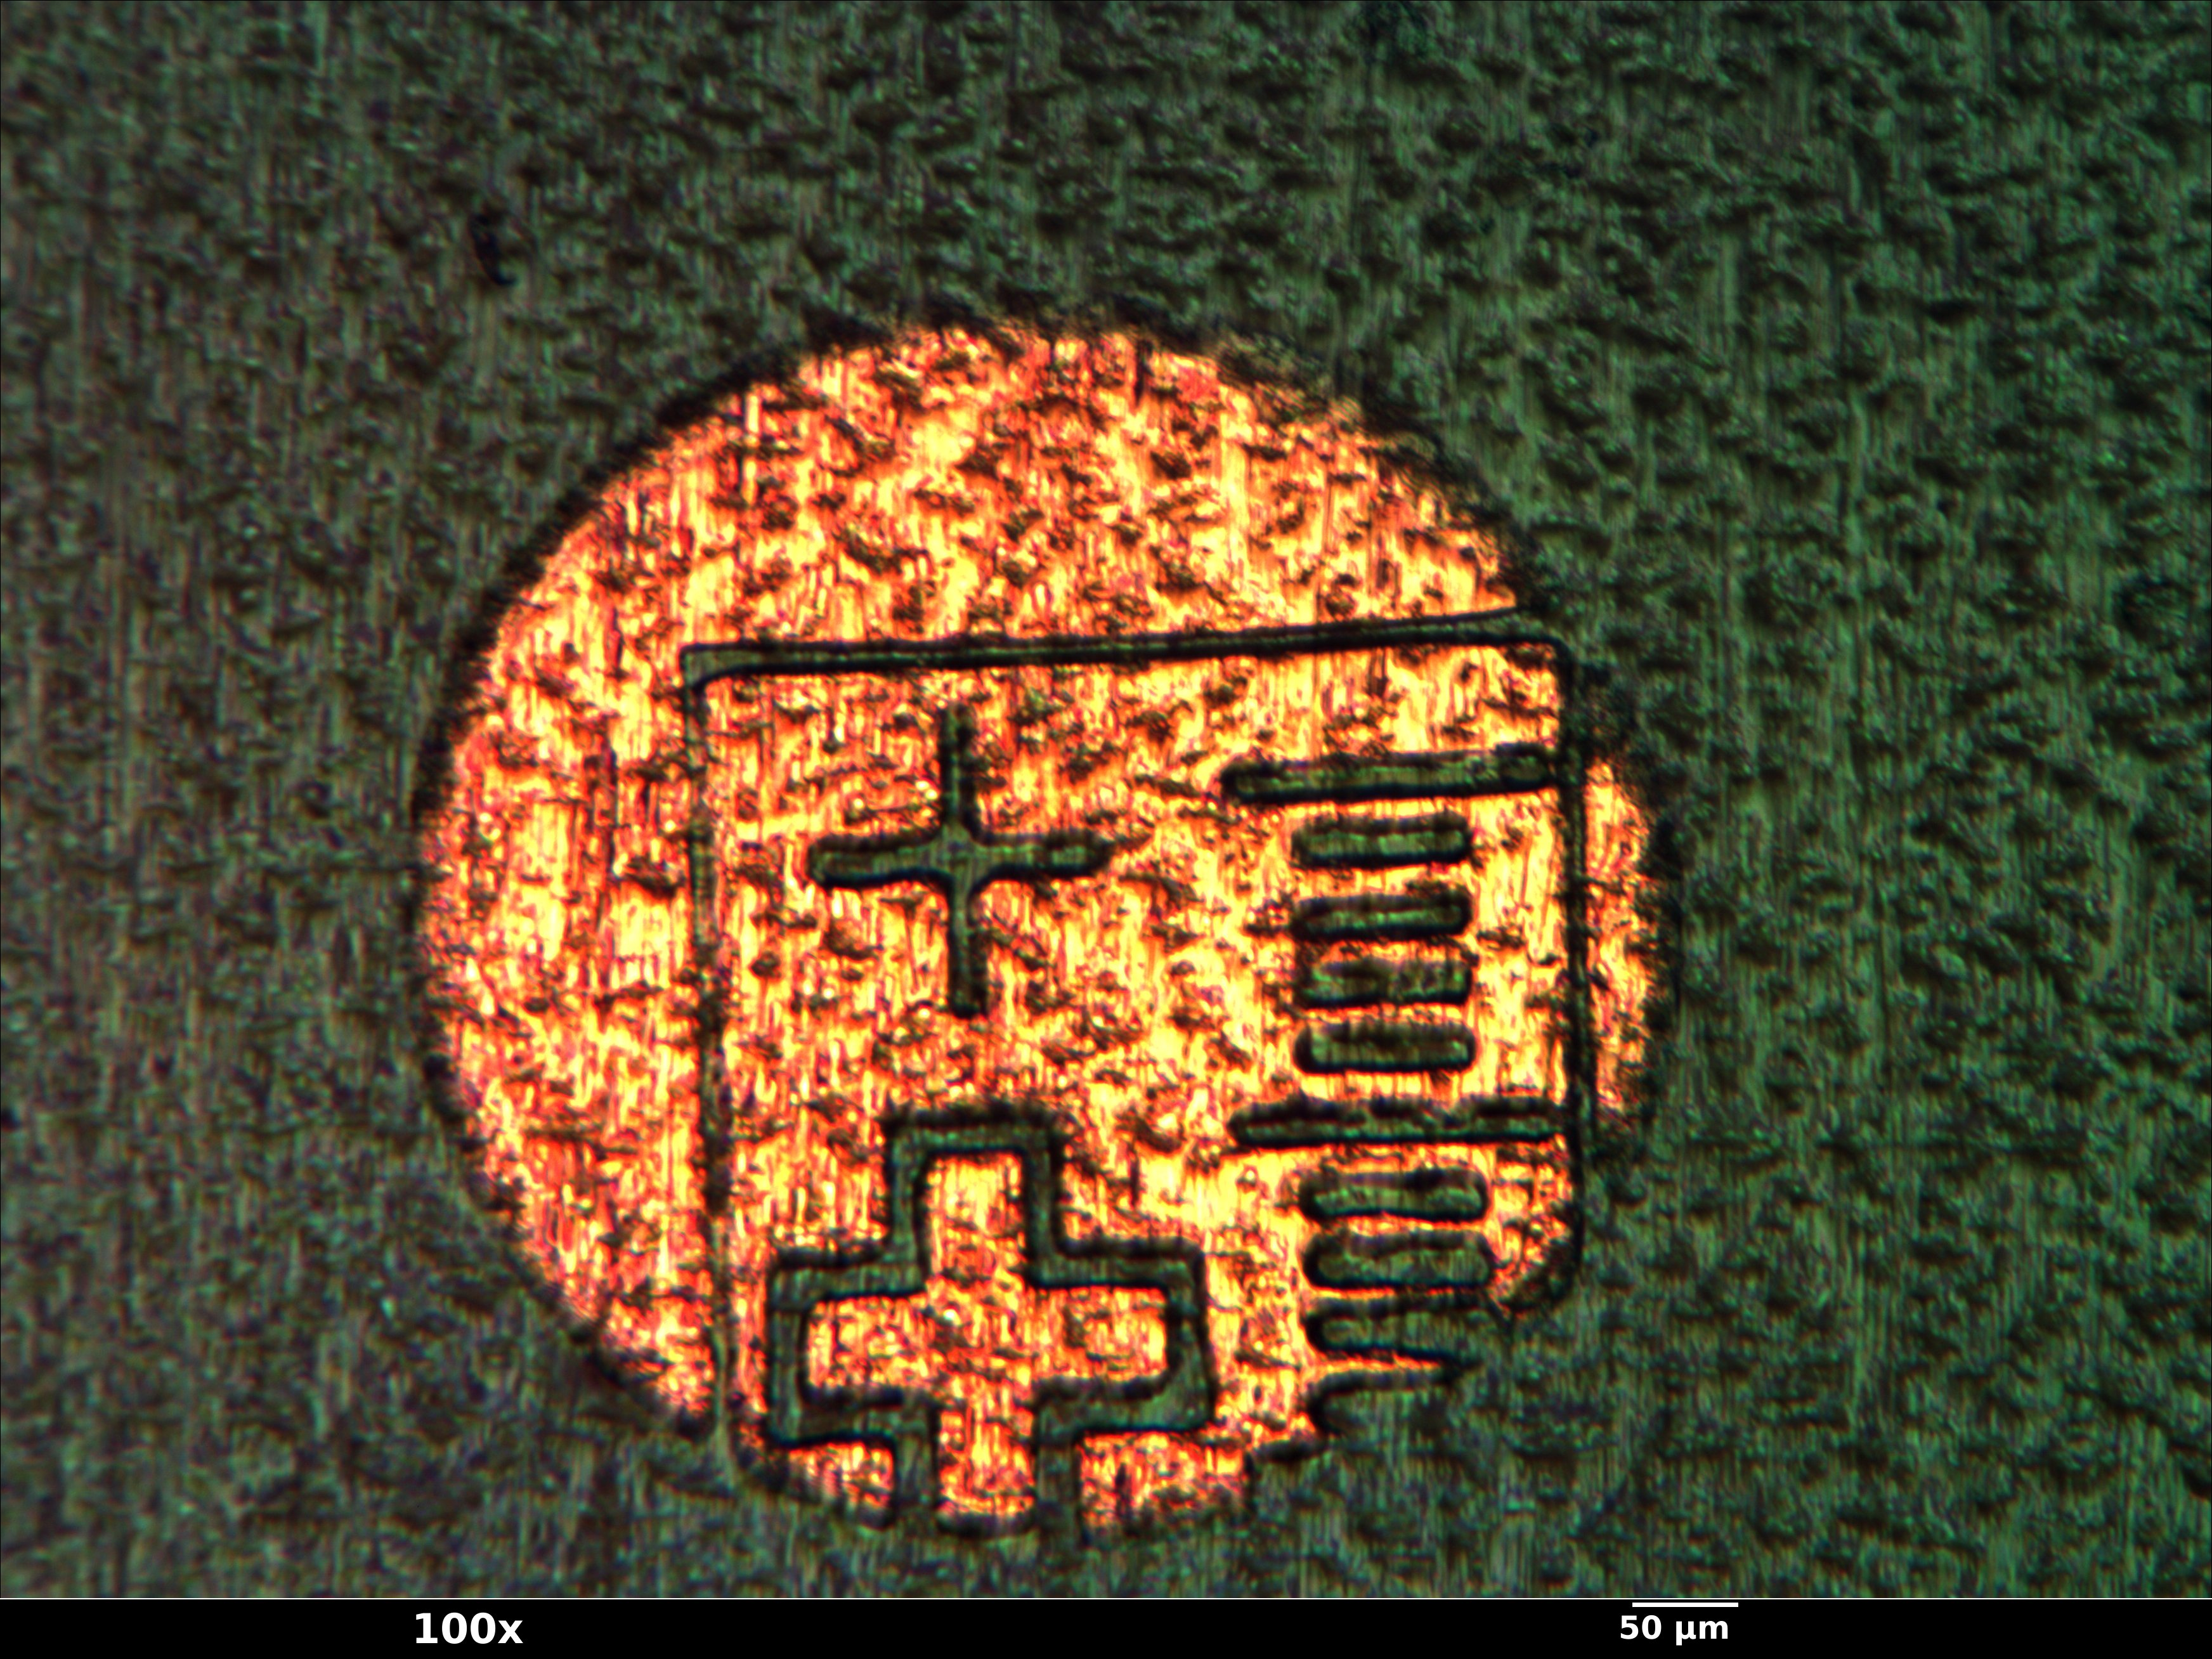
\includegraphics[scale=0.06]{mask011_annotated.jpg}
\end{center}
\caption{Lower magnification view of sample.}
\label{lowmag}
\end{figure}

\begin{figure}[h!]
\begin{center}
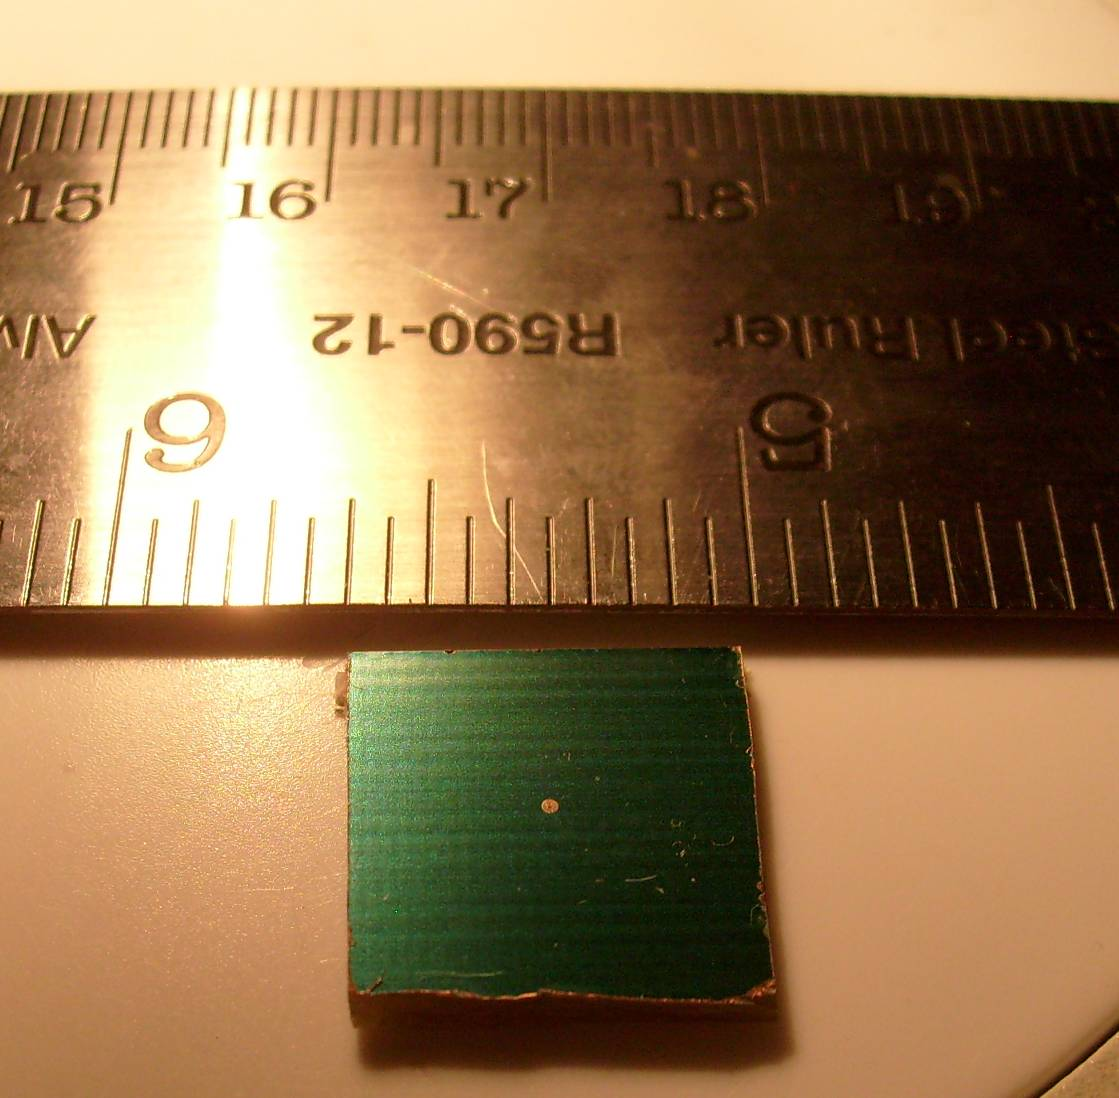
\includegraphics[scale=0.2]{actual-size.jpg}
\end{center}
\caption{Unmagnified view of sample}
\label{actual}
\end{figure}

\paragraph*{}
After developing the sample was inspected under the microscope with mask art still in place. Fig. ~\ref{alignment-1} 
shows the initial view after focusing the image. Note that the outer alignment mark is on the substrate; in an actual
multi-level mask design the inner mark is typically placed on the substrate.

\paragraph*{}
The sample was then aligned to the projected mask using stage motion controls. Achieving alignment of better than 5-10
$\mu m$ was not difficult. 

\paragraph*{}
The final patterns were measured using a camera which had been previously calibrated with a stage micrometer. Actual
half-pitch of $200 \mu m$ half-pitch mask patterns projected using the 40x objective was slightly under $15 \mu m$.

\section{Conclusions}
\paragraph*{}
A method for converting a metallurgical microscope into a projection mask aligner for photolithography is demonstrated.
The method requires little specialized equipment and all modifications are reversible. General functionality of the
microscope is not significantly degraded by the modifications. Features as small as $15 \mu m$ were fabricated in
positive photoresist on copper substrates.

\paragraph*{}
It is the author's hope that this and future techniques will raise interest in microfabrication, nanotechnology, MEMS,
and related fields among hobbyists.

\section{Future work}
\paragraph*{}
Actual etching of developed substrates was not performed due to the substrate used in these experiments ($35 \mu m$ Cu
with a rough surface finish). Without anisotropic etch capabilities for Cu, patterning these substrates is not feasible.

\paragraph*{}
The tests performed in this paper used professionaly coated dry-film photoresist. The author also has a can of
Shipley Photoposit SP24 photoresist (which has been successfully spin-coated onto metallic substrates in previous tests)
and intends to test its performance on polished Si wafers in the near future. When used to pattern a spin-on-glass or 
thermal oxide hard mask, followed by a KOH-IPA anisotropic wet etch, it should be possible to create $15 \mu m$ features
in silicon.

\paragraph*{}
The method used in experiment 1 has not been fully explored, and appears to offer the capability of creating
significantly smaller features than that of experiment 2. Given a properly collimated and uniform light source, it is
expected to prove far superior to the second method.

\paragraph*{}
The field of view of the current system is rather limited, especially method 2. (see Fig. ~\ref{lowmag} and Fig.
~\ref{actual}). The author intends to explore a scanner- based system which will move the mask and substate at the
correct speed ratios to pan a larger mask over the lens and allow dies larger than a $37 \lambda$ disk to be made. This
will require precise stage control and a more intense illuminator than the current system has to ensure reasonably short
exposure times.

\paragraph*{}
The microscope used in tests is equipped with a 100x oil immersion objective. If a suitable refractive medium can be
found (which does not interfere with the normal exposure/development process) there is a possibility of significantly
smaller features - up to $6 \mu m$ with method 2 or $2 \mu m$ with method 1.

\section{Acknowledgements}
\paragraph*{}
The author wishes to thank Dane Kouttron, John McMaster, and the other members of the RPI Electronics Club for useful
suggestions during his early photolithography work, which paved the way for this research.

\begin{thebibliography}{99}
	\bibitem{ellsworth}
	Jeri Ellsworth, ``Home Chip Fab", Available: http://makerfaire.com/pub/e/2545

\end{thebibliography} 

\end{document}
